\documentclass[a4paper,12pt]{article}

\usepackage[utf8]{inputenc}
\usepackage[ngerman]{babel}
\usepackage[T1]{fontenc}
\usepackage{graphicx}
\usepackage[cache=false]{minted}
\usepackage{dirtree}

\begin{document}
\begin{titlepage}
    \begin{center}
        \vspace*{1cm}
        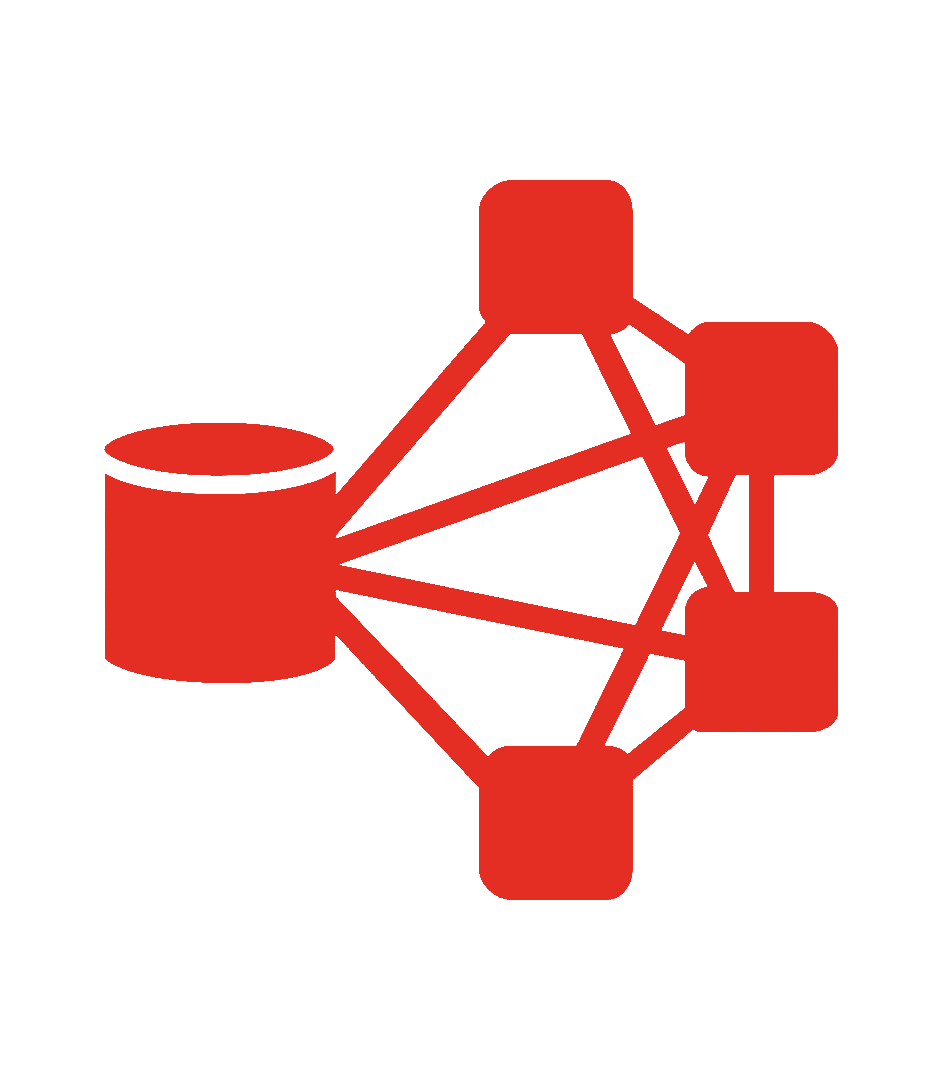
\includegraphics[width=10cm]{Logo.png}
        
        \textbf{\huge MapReduce-System}
        
        \vspace{0.5cm}
        NVS Projekt 2
                 
        \vspace{1.0cm}
    
        \textbf{Alexander Grill 5CHIF}
        
        \today
        
        \vfill
                 
                 
        \vspace{0.5cm}
                 
        Informatik\\
        HTBLUvA Wr.Neustadt\\
        Österreich\\

                 
    \end{center}
\end{titlepage}  
\newpage
\tableofcontents
\newpage


\section{Einführung}
In diesem Kapitel werden die Gründe der Umsetzung und das Thema, worum es in dieser Arbeit geht, genau erläuter. Es wird auch
darauf eingegangen, welche Thematiken das Projekt umfassen soll und wie sich die Benotung auseinander setzt.

\subsection{Vorwort}
Der Virus "COVID-19" war im Jahr 2020 für die gesamte Bevölkerung auf der Erde eine rießengroße Herausforderung. Die Situation änderte sich am Begin im daruffolgendem Jahr 2021 nicht, 
deshalb beschloss die Bundesregierung weiter Maßnahmen, Ausgangsbeschränkunge, Grenzkontrollen, FFP2-Maskenpflicht und weitere Regeln die, die Bevölkerung einzuhalten hat. Alle Schüler in Österreich müssen die Schule 
blockweiße besuchen. Nur mit einem davor verpflichtetenden Schnelltest und FFP2-Maske dürfen sie die Schule betrehten. Da die Projektarbeiten im ersten Semster dementsprechend gut ausgefallen sind, beschloss Herr Professor 
Kolousek, dass Schüler in den fünften Klassen im Fach NVS statt der Praktischen Arbeit und dem Theorie Test eine Projektarbeit über den Semsterstoff machen müssen. Folgendessen muss die Dokumentation, über das gewählte Thema, dementsprechend einen
weiteren Umfang umfassen als beim ersten Projekt im ersten Semster. Im praktischen Teil geht es in diesem Projekt, darum ein Map-Reduce System in Kombination mit Server-Client Kommunikation zu implementier. Im theoretischen Teil, werden die Grundlagen die für die 
Umsetzung relevant sind erklärt. Zusätzlich beinhaltet dies auch sämtliche Abschnitte wie, die Source Code Dokumentation, Abläufe, Erklärung bezgl. MapReduce-System, Aufbau und Anwendungsfälle.
\begin{description}
    \item[Die zu erreichende Note hängt prinzipiell von der] ~\par
    \begin{itemize}
        \item Beispielkategorie
        \item Art der Kommunikation
        \item Funktion, Umfang und Tiefe der Implementierung
        \item Fehlerbehandlung
        \item Ausgaben, Einhaltung der Coding Conventions, Kommentare
        \item Repository: Commits, Issues
        \item Ausarbeitung
        \item Einhaltung der Richtlinien
      
    \end{itemize} 
\end{description}
\subsection{Motivation}
In diesem NVS Projekt geht es darum, ein MapReduce-System mit der Programmiersprache C++ unter Linux mittels g++ Compilier umzusetzten.
Im kurzem zusammengefasst soll eine große Menge an komplexen, unstrukturierten und eine Art von aufwendigen Daten verarbeitet werden. 
Das heißt es sollen Daten, die planlos abgespeichert sind, zusammengefasst werden, sodass diese wieder ihren Nutzen oder Sinn erbringen. Diese können
dann für weiter Verarbeitungsschritte oder Datenanalysen verwendet werden. Die Daten werden am Beginn in kleiner Packete aufgeteilt und diese werden identifiziert mit einem eindeutigen
Schlüssel. In der nächste Phase werden die einzelnen Packete parallel von unterschiedlichen, getrennten und unabhängigen Prozesse zusammengefasst. Danach werden die gruppierten Daten wieder 
einen Schlüssel zugeordnet, sodass diese wieder zusammengefasst und minimiert werden. Die Kommunikation zwischen den einzelnen Knoten, soll in dieser Arbeit mittel Server-Client Kommunikation passiern.
Der Server hört auch einem Port ab, ob sich ein Client damit verbinen möchte, wenn eine Verbindung aufgebaut werden kann, soll die Splittung der Daten passier, daraufhin soll das Resultat weiter an dem Server gegeben werden, bis 
alle Daten vereint auf dem Master Server liegen. Die bearbeitetn Daten werden schlussendlich in einem JSON-File abgespeichert.
\section{Aufgabenstelllung}
Diese Kapitel umfasst die genaue Erläuterung der Aufgabenstelllung, als auch die Themenbereiche die dieser Projektarbeit. Darüber hinaus wird auch über die Idee der Umsetzung geschrieben.

\subsection{Erläuterung der Aufgabenstellung}

\subsection{Idee}

\subsection{Themenbereiche}
\newpage
\section{Grundlagen}

\subsection{Was ist ein MapReduce System?}
Das Verfahren wurde 2004 von Google entwickelt für die Indexierung von Webseiten. Das Framework wird bei Datenbanken eingesetzt und dient zur Verarbeitung von großen, komplexen, unstrukturierte Datenmengen.
Dieses Verfahren findet Anwendung für BigData und Datawarehouse, weil in solchen Fällen große Datenmengen in kürzester Zeit mittels Software verarbeitet, analysiert, aggregiert als auch kompremiert werden. 
Map Reduce parallelisiert die Bearbeitung, durch die Verteilung auf mehrere gleichzeitig auszuführende Tasks. Der Grund, warum dieses Framework solche Datenmengen verarbeiten kann ist, weil die Aufgaben auf mehreren Rechnern aufgeteilt werden. Jeder einzelne Rechner startet Prozesse, die Parallel die Daten verarbeitet und auswertet.
Ein einzelner Rechner stoßt schnell an seine Grenzen, deshalb ist die Verarbeitung von Daten, mittels mehreren Knoten sehr effizient und bietet eine bessere Performance.
Das Verfahren wurde in vielen verschiedenen Verfahren eingesetzt wie zum Beispiel für die Indizierung von Webseiten, nach einer Suchanfrage mit beliebigen Zeichenketten, ebenso im Umfeld von Google News wird MapReduce verwendet. Andere große Internetfirmen wie Yahoo, die ebenfalls das Verfahren für die Indexierung von Webseiten verwenden, 
als auch Facebook verwendet das System, um Spam Messages zu minimierung und die Ads zu optimieren. Wohingegen Amazon das Verfahren für das Clustering der Produket verwendet

\subsection{Map und Reduce}
Die beiden Grundfunktionen des Verfahrens sind Map und Reduce. Sie sorgen für die Aufteilung der Aufgaben in kleinere parallelisierten Arbeitspakete und führen am Ende die Ergebnisse zusammen. Bei großen relationalen Datenbanken und komplexen Queries lassen sich typische Problem, bezglüch Verarbeitung von großen Datenmengen beseitigen.
Die Map Funktion, verteilt die Aufgaben an unterschiedlichen Knoten eines Clusters. Die Reduce Funktion sortier die verfassten Ergebnisse und fügt sie am Ende wieder zusammen.
Die Funktionen Map und Reduce werden vom User bereitgestellt, weil diese schließlich zu den bereitgestellten Daten passen müssen.
\newpage

\subsection{Ablauf}

\begin{figure}[h]
    \centering
    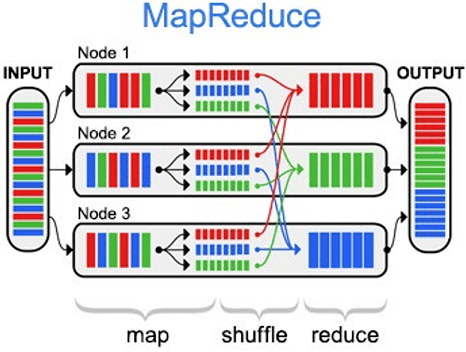
\includegraphics[width=6.1cm]{mapreduce.png}
\end{figure}

\begin{description}
    \item[Das Verfahren verläuft durch folgende Schritte:] ~\par
    \begin{itemize}
        \item Split
        \begin{itemize}
            \item{Die bereitgestellten Daten werden aufgeteilt. Jeder Datensatz darin ist identifiziert durch
            einen Schlüssel-Wert. Diese Datenmenge wird nun in kleinere Datenmengen aufgeteilt
            und vom Master an die verfügbaren Knoten verteilt.}
        \end{itemize}
        \item Map 
        \begin{itemize}
            \item{Nun wendet jeder Knoten auf die Daten die Map-Funktion an, die schließlich Key/Value Paare zurückgibt. Diese Ergebnisse werden zwischengespeichert.}
        \end{itemize}
        \item Shuffel
        \begin{itemize}
            \item{Bei diesem Schritt geht es darum den reduce-Knoten, die entsprechenden Daten zuzuteilen.
            Diese Zuteilung entspricht einer Fragmentierung.
            Hierbei wird den Knoten, die reduce ausführen, ein Key zugeteilt. Diese Knoten holen sich
            dann die bereits durch Map entstandenen Datensätze mit diesem Key und wenden reduce an.}
        \end{itemize}
        \item Reduce
        \begin{itemize}
            \item{Grundsätzlich ist die Aufgabe dieser Funktion, die Key/Value Paare anhand des Schlüssels
            zusammenzufassen und dabei die Summe der einzelnen Values zu bilden. Demnach ist die
            Ausgabe der Reduce-Funktion wieder ein Key/Value Paar mit dem gleichen Aufbau wie vor
            der Verarbeitung.
            Dies ermöglicht es, dass reduce mehrere Male angewendet werden kann, bis schließlich alle
            Daten gesammelt wurden.}
        \end{itemize}
    \end{itemize} 
\end{description}

\subsection{Vorteile Nachteile eines Map-Reduce Systems}
Map Reduce bietet eine Menge an Vorteilen, gegenüber den klassischen Verfahren der Datenverarbeitung, wie
sie in den relationalen Datenbanksystemen verwendet werden. \\ \\
Ein wesentlicher Vorteil ist, dass für die
Verwendung eines solchen System ein einfacher normaler Rechner benötigt wird und keine Highend-Server. Ein Cluster-Verbund für die parallelisiert
Datenverarbeitung kann bei Notwendigkeit ohne großen Aufwand realisiert werden. Ein Cluster-Verbund ist ein Netzwerk, das aus mehreren Rechner besteht die gleichzeit miteinander verbunden sind 
und sich Daten austauschen. Aus diesem Grund ist ein MapReduces-System sehr kostensparsam und kann mit wenig Know-How und Erfahrungen umgesetzt und
schlussendlich in Verwendung gebracht werden. \\ \\
Ein weiterer Vorteil ist auch die Skalierbarkeit. Da die Daten auf den jeweiligen Knoten
aufgeteilt werden, bietet das System eine zuverlässige Ausfallstoleranz und Verfügbarkeit, denn wenn ein Knoten ausfallen sollte, werden die Daten einfach an einem
anderen Knoten und dort verarbeitet, somit läuft das System zu jederzeit in einem stabilen Zustand. \\ \\
Durch die parallelisierte Verarbeitung von Daten ist dieses Verfahren deutlich effizienter und perfomanter als die Datenverarbeitung
in relationalen Datenbanken. Im Terabyte-Bereich dauert das Verfahren oft nur Minuten, im Petabyte-Bereich Stunden, wobei andere Systeme deutlich mehr Zeit und Ressourcen für die Verarbeitung
benötigen.\\ \\
Während die Berechnungen schnell gehen, dauert der Datenzugriff länger als bei anderen Methoden. 
Die Daten müssen erst über das Netzwerk gestreamt werden. Dabei ist die Netzanbindung der Flaschenhals, vor allem im Hinblick auf die sehr unterschiedlichen Rechner innerhalb des Clusters und deren unterschiedliche schnelle Netzanbindung.\\ \\
Um die Geschwindigkeit zu erhöhen, kann ein Cluster ausschließlich aus High-End-Servern bestehen. In diesem Fall sind die Kosten für das MapReduce-Verfahren immens hoch.





\section{Umsetzung}

\subsection{Aufbau}

\subsection{Klassendesign}

\subsection{Source Code Dokumentation}

\subsection{Verwendete Bibliotheken}

\section{Anwendungsfälle}

\section{Schlusswort}

\end{document}
